\chapter{Application de quelques technologies Big Data sur l'analyse des traceroutes} \label{chap:application-on-traceroutes}


\section{Introduction}

Ce chapitre reprend un ensemble de   technologies destinées  à la manipulation des données massives. Ce sont les technologies que nous avons expérimenté pour analyser des traceroutes disponibles dans le dépôt de RIPE Atlas. Précisément, ce sont les traceroutes permettant de tracer l'évolution du délai d'un lien comme il décrit le chapitre \ref{chap:big-data-intro}.
% Nous allons présenter l'objectif de chaque technologie, ses avantages, ses inconvénients et ses limitations dans le cas de la présente analyse.
%Le présent chapitre reprend l'application de quelques technologies du Big Data manipulées en vue d'analyser le délai des liens. 
%On ne peut pas comparer ces technologies entre elles car elles ne se trouvent pas dans la même catégorie; quelques technologies n'assurent que le stockage, une autre technologie gère l'analyse ainsi que le stockage.  En revanche,
Les technologies que nous présentons  couvrent les besoins d'une ou de plusieurs étapes d'un processus d'analyse de données.
% (voir un exemple d'un processus d'analyse de données dans la section \ref{sec:process-data-analysis}). 
 
 %L'évaluation des performances  des technologies choisies est faite sur une machine ayant les caractéristiques reprises dans le tableau[!].

\section{Critères d'évaluation des technologies  Big Data}

Les critères d'évaluation d'une technologie Big Data par rapport à une autre dépendent de plusieurs entrées.  En générale, la liste des critères que l'on peut considérer dans la comparaison des technologies Big Data entre elles est très longue.  En ce qui concerne les critères sur lesquels nous  évaluons  les différentes technologies  Big Data sont les suivants:
\begin{itemize}
\item configuration de l'environnement de la technologie Big Data;
\item flexibilité liée à la définition du  schéma de  données présentes dans les fichiers de données;
\item temps d'exécution nécessaire pour fournir les résultats finaux d'une analyse de traceroutes lancée;
\item évolutivité de l'environnement Big Data mis en place pour des nouvelles données et de nouveaux besoins.

\end{itemize}
En pratique, nous n'avons pas pris en compte d'autres critères dans notre cas, car nous ne pouvons pas les évaluer. Par exemple, l'utilisation du  Big Data engendre des coûts  liés aux ressources nécessaires au stockage de données massives ainsi qu'au traitement de ces dernières. Nous avons donné des indications sur les frais d'utilisation de deux technologies dédiées au stockage de données massives : Amazon S3 (voir le Tableau \ref{tab:pricing-s3-standard}), alors que les frais d'utilisation de MongoDB Atlas dépend de plusieurs paramètres. 

\section{Caractéristique de l'environnement de test}

Les différents tests ont été réalisés sur un conteneur de type OpenVZ ayant les caractéristiques suivantes : conteneur OpenVZ, système Debian GNU/Linux 7.11 (wheezy),  32768 MB de  RAM,  CPU  modèle $6$, CPU MHz $ 2294.331 $.

%Le Tableau \ref{tab:test-machine} présente les caractéristique de la machine sur laquelle nous avons effectué les différents tests. 
%\begin{table}[H]
%	\begin{tabular}{cc}
%		Type& OpenVZ container\\
%		RAM (MB)& 32768 \\
%		CPU & 64 (The logical CPU number of a CPU as used by the Linux kernel) \\
%	\end{tabular}
%	\caption{Caractéristiques de la machine de test}
%	\label{tab:test-machine}
%\end{table}


\begin{tcolorbox}
	
	Il existe différentes catégories de virtualisation, \textbf{OpenVZ} s'inscrit dans la catégorie Isolateur. Un isolateur est un logiciel permettant d'isoler l'exécution des applications dans des contextes ou zones d'exécution. Un conteneur OpenVZ s'agit d'un partitionnement logique au niveau des ressources systèmes : processus, réseau et système de fichier\footnote{Source : \url{http://cesar.resinfo.org/IMG/pdf/jtsiars-openvz_1_.pdf}, consultée le $29/12/2018$.}.
\end{tcolorbox}


\section{Application 1 : MongoDB}
%\paragraph{ Application sur  MongoDB}~

%Les données relatives aux mesures traceroutes peuvent être récupérées de différentes manières. Par exemple,  les traceroutes à destination des instances du serveur DNS K-root. En ce qui concerne le travail de référence, les traceroutes sont récupérés à la fois par type d'adressage : IPv4 et IPv6 en se basant sur  l'identifiant  de la mesure : $ 5001 $, $ 6006 $, etc et par date.  Ainsi les
MongoDB est la technologie Big Data utilisé par  Fontugne  dans l'implémentation de l'outil de détection \cite{InternetHealthReport}. Dans MongoDB, les traceroutes sont organisés  dans des collections.  Chaque collection stocke les traceroutes effectués lors de la journée $YYYY\_MM\_DD$ et en adressage $V$. Dans le  cas de l'adressage IPv4, $V$  ne prend aucune valeur,  or, $V$ prend la valeur $6$ s'il s'agit de l'adressage IPv6.  La nomination structurée des collections permet de ne récupérer que les traceroutes concernés par l'analyse lancée. Le nom d'une collection est structuré comme suit: 	$tracerouteV\_YYYY\_MM\_DD$.
 

 
 MongoDB est une technologie conçue pour assurer  le stockage de données dans un processus d'analyse de données. Nous avons utilisé la version locale de MongoDB, la quantité de données que nous pouvons stocker ainsi que le traitement de données récupérées dépend principalement des ressources de la machine dans laquelle MongoDB est installé.
 
    MongoDB est flexible en terme de définition du schéma de données; aucun schéma n'est requis.   Par exemple, dans certains cas, les traceroutes planifiés ne réussissent pas à atteindre une destination, dans ce cas le contenu d'un traceroute est différent de celui réussi. 
    
    Généralement l'analyse de données à grande échelle se limite qu'au mode lecture de données pour en tirer les connaissances. MongoDB est adapté non seulement aux projets visant la lecture de données massives mais aussi aux projets où on envisage la mise à jour d'un objet dans une collection (modification ou suppression). 
 
 En cas de la  mise à jour de la structure de données des objets traceroutes par RIPE Atlas,  cela n'affecte pas la solution mise en place avec MongoDB. 
 
 %Malgré la convenance de MongoDB aux données non structurées et massives, l'utilisation de telle base de données, en version locale, nécessite l'ajustement de la machine locale où MongoDB tourne. 



%\paragraph{Les limitations de MongoDB}

%L'implémentation proposée de l'outil de détection utilise la version locale de la base de données MongoDB pour le stockage des données.  La quantité de données dont MongoDB peut stocker dépend de l'espace mémoire de stockage disponible dans la machine dans laquelle MongoDB est installé. De plus, les performances d'une détection lancée concernant une période donnée dépendent de la RAM de la machine en question. Pour conclure, l'utilisation de la version locale d MongoDB pour analyser les traceroutes à travers l'outil de détection dépend typiquement de la machine locale.

%\paragraph{Les performances de MongoDB}




\paragraph{Performances de la base de données MongoDB dans l'analyse des délais }~

Nous évaluons les temps d'exécution lors de l'analyse des délais en utilisant MongoDB comme technologie de stockage de données massives.  Dans le Tableau \ref{tab:mongotiming-timing}, nous varions la quantité de données analysées pour mesurer le temps nécessaire pour avoir  l'évolution de tous les liens présents dans  les traceroutes analysés. 

\begin{table}[H]
	%\begin{threeparttable}
	
	\captionsetup{justification=centering}
	\begin{tabular}{ccccc}
		\textbf{Début - fin} &\textbf{Durée (jours)}  & \textbf{Taille}  & \textbf{Nb traceroutes} & \textbf{Temps (secondes)} \\ \hline
		
		07/02/2018             &1 &1 GB&& 3870\\ \hline
		07/02/2018 - 08/02/2018&2 &1 GB&& 2942\\ \hline
		07/02/2018 - 09/02/2018&3 & 1 GB&& 2991\\ \hline
		07/02/2018 - 10/02/2018&4 & 3 GB&& 20955\\ \hline
		07/02/2018 - 11/02/2018&5& && \\ \hline
		07/02/2018 - 12/02/2018&6& && \\ \hline
		07/02/2018 - 13/02/2018&7& && \\ \hline
		07/02/2018 - 14/02/2018&8& && \\ \hline
	    07/02/2018 - 15/02/2018&9& && \\ \hline
	    07/02/2018 - 16/02/2018&10& && \\ \hline
	    07/02/2018 - 17/02/2018&11& && \\ \hline
	    07/02/2018 - 18/02/2018&12& && \\ \hline
	    07/02/2018 - 19/02/2018&13& && \\ \hline
	    07/02/2018 - 20/02/2018&14& && \\ \hline
	\end{tabular}
	\caption{La moyenne des temps d'exécution d'analyse de traceroutes en fonction de la taille de données avec MongoDB}
	\label{tab:mongotiming-timing}
\end{table}


\section{Application 2 : Amazon DynamoDB}


%\paragraph{Application sur les traceroutes}~


L'élasticité est une des caractéristiques attirantes des services web d'Amazon. En particulier, c'est le cas d'Amazon DynamoDB. Une implémentation basée sur Amazon DynamoDB  n'a pas à se soucier de la capacité  de stockage de données.

 Amazon DynamoDB  n'assure que le stockage de données dans un processus d'analyse de données. La récupération et le traitement  des données stockées nécessite l'ajustement des ressources de la machine qui reçoive ces données, pareillement à MongoDB. La différence se situe à l'évolutivité implicite du stockage de données, qui ne se limite que par la capacité de stockage physique d'AWS. Tandis qu'une installation locale de MongoDB est liée aux ressources de la machine hébergeant ce dernier.  Nous n'avons pas expérimenté Amazon DynamoDB pour analyser les traceroutes, étant donné que notre évaluation des temps d'exécution est effectuée sur une machine locale, nous aurons les même remarques que dans le cas de MongoDB en ce qui concerne l'ajustement des ressources de la machine qui reçoive les données.  
 
 A titre indicatif, une heure de tous les traceroutes effectués par toutes les sondes Atlas fait une taille moyenne de  $620$ MB en format compressé, ce que représente une quantité d'environ $9$ GB en format texte.


%Toutefois,  au moment de de la récupération et de la manipulation de ces données, il faut ajuster les ressources pour pouvoir récupérer et traiter une quantité importante de données.




\section{Application 3 : Amazon S3, Amazon Glue  et Amazon Athena }


%\paragraph{Application sur les traceroutes}~

Nous avons combiné les trois services d'Amazon (Amazon S3, Amazon Glue  et Amazon Athena)  afin de créer un environnement d'analyse de données massives. Une vue globale du  processus de l'analyse  est illustré dans la Figure \ref{fig:gluecrawler}\footnote{Amazon Redshift  est un entrepôt de données et et  Amazon Quicksight  est un service cloud d'informatique décisionnelle.}. 

\begin{figure}[H]
	\centering
	\captionsetup{justification=centering}
	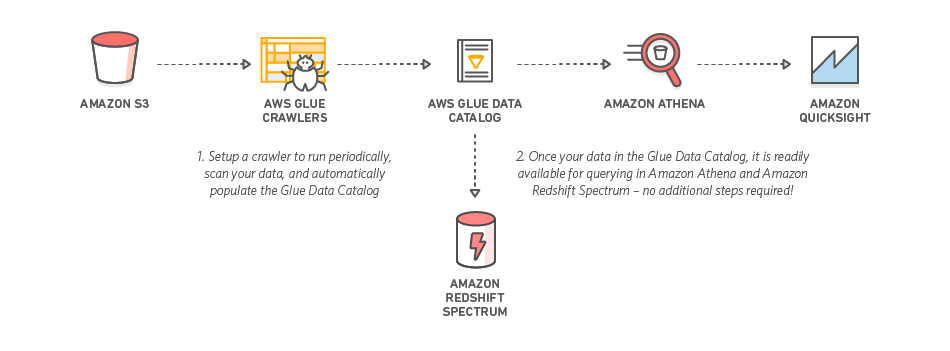
\includegraphics[width=1\linewidth]{illustrations/glue_crawler}
	\caption{Une combinaison des services web d'Amazon : Amazon S3, Amazon Glue, Amazon Athena, Amazon Quicksight  et Amazon Redshift}
	\label{fig:gluecrawler}
	\source{\url{https://docs.aws.amazon.com/fr_fr/athena/latest/ug/glue-best-practices.html}, consultée le $16/12/2018$.}
\end{figure}


Afin d'utiliser Amazon Athena, nous avons besoin du schéma de données. Il s'agit d'une table comme les tables dans un SGBDR. Pour ce faire, 
nous avons lancé  avec Amazon Glue  la détection automatique du schéma d'un ensemble de  traceroutes enregistrés dans un fichier faisant une taille de $500$ MB. Toutefois, la détection a échoué. Autrement dit, Amazon Glue n'a pas pu inférer le schéma d'une seule table capable de lire tout traceroute dans ce fichier.  L'échec de l'inférence est dû au fait que le fichier contient des traceroutes différents en terme de structure, car la structure dépend du firmware de la sonde ayant effectué le traceroute.
 %L'origine de cette différence  est le fait que ces traceroutes ont été effectués par des sondes ayant un firmware différent. Car le contenu des résultats d'une requête traceroute  et son organisation dans un objet JSON dépend partiellement du firmware de la sonde. 
 Pour finir, le schéma des traceroutes a été créé manuellement (voir la section \ref{creer-table-traceroute} dans l'annexe \ref{athena-appendix}). La table a été créée en utilisant le partitionnement des données dans un compartiment S3. Plus de détails sur le partitionnement sont données dans la section \ref{subsubsection:partitionnement} dans l'annexe \ref{athena-appendix}.


Une fois les fichiers de données sont synchronisés vers le compartiment AWS S3 et le schéma  de données est créé, on passe à l'interrogation de données en utilisant les requêtes SQL basées sur Presto.  

Pour intégrer Amazon Athena dans l'outil de détection \cite{InternetHealthReport}, on distingue deux possibilités. La première possibilité n'utilise Athena que pour récupérer, dans la machine locale,  les traceroutes vérifiés en terme de validité; c'est l'objectif des étapes $1$ et $2$ dans le processus de la création de l'évolution des RTTs différentiels des liens (voir la section \ref{steps-rtt-analysis}).  Les traitements qui suivent (étapes  à partir de $3$) sont effectués dans la machine locale. Dans ce cas, l'utilisation des technologies  Big Data est limité qu'au niveau stockage de données massives. 

Tandis que  la deuxième possibilité vise la maximisation des traitements au sein de l'infrastructure  d'Athena. De ce fait, la machine locale n'a qu'à recevoir les derniers résultats de la détection, voire les résultats finaux. Pour cette deuxième possibilité, les données doivent être manipulées de sorte à maximiser,  	au niveau d'Amazon Athena,  les traitements relatives à toutes les étapes décrites dans la section \ref{steps-rtt-analysis}. 

Pour la deuxième possibilité, le défi est de trouver la requête ou bien l'ensemble de requêtes SQL à exécuter sur Athena en vue d'avoir l'évolution du RTT différentiel des liens. 
Vue la complexité des  étapes $1$ à $9$, on ne peut pas trouver une seule requête SQL assurant toutes les étapes. Supposons qu'il existe une requête SQL capable de trouver les liens possibles avec leurs RTTs différentiels : à l'étape $ 4 $ dans \ref{steps-rtt-analysis}, on construit la distribution des RTTs différentiels pour tout lien $l$ identifié dans les traceroutes de la période $d_k$. Cette distribution est mise à jour à chaque fois $l$ est identifié dans un des traceroutes  de la période $d_k$. Soient  $T_k$ = \{$t_{k, j}$\}  l'ensemble de traceroutes effectués durant $d_k$, avec $j \in [1, R]$ et R est le nombre de traceroutes effectués durant $d_k$. Nous décrivons le parcours des traceroutes d'une période $d_k$ brièvement dans le pseudo-code \ref{alo-inference-link}, sachant que les détails ne sont données, l'objectif est d'évaluer la convenance d'Athena au traitement souhaité.
\begin{algorithm}[H]
\begin{algorithmic}[1]
	 \ForAll{ $t_{k, j}$ $\in$ $T_k$} \
	  \State $links$ $\leftarrow$ getLinksFromTraceroute($t_{k, j}$)
	  	 \ForAll{$l$ $\in$ $links$}
	  	 		\State updateLinkRttDistribution($l$) \label{update-link}
	  	 \EndFor
	 \EndFor
\end{algorithmic}
\caption{Une partie de l'étape $4$ du processus de la détection des anomalies des délais }
\label{alo-inference-link}
\end{algorithm}

Avec : 
\begin{itemize}
	\item \textit{getLinksFromTraceroute($t_{k, j}$)} énumère tous les liens possibles dans le traceroute $t_{k, j}$.

    \item \textit{updateLinkRttDistribution($l$)} ajoute le RTT différentiel calculé du lien $l$ à la distribution des RTTs différentiels courante de ce lien pour la période $d_k$.
\end{itemize}


Le service Athena est conçu pour la lecture de données, toute mise à jour de données n'est pas possible avec ce service. C'est pourquoi la distribution des RTTs différentiels de chaque  lien identifié doit être sauvegardée dans un endroit accessible en lecture et en écriture, par exemple dans un compartiment AWS S3. Que ce soit un fichier reprenant la distribution des RTTs différentiels  par un seul lien ou bien un fichier pour tous les liens,   à la ligne  \ref{update-link} du pseudo-code \ref{alo-inference-link}, un fichier doit être lu et mise à jour avec de nouvelle valeur. Pour une période $d_k$ d'une heure, le nombre de traceroutes est de l'ordre de milliers. Chaque traceroute peut inclure $L$ liens. Dans ce cas, le nombre total, d'une période $d_k$, de mise à jour de la distribution des RTTs différentiels est de l'ordre $R$\texttimes$L$ de fois.  Cette estimation est à titre indicatif, de plus elle ne concerne que l'étape $4$, le nombre de lectures et/ou d'écritures dépend des requêtes SQL créées pour les autres étapes. 

En plus du nombre de lectures et d'écritures, la détection des anomalies repose sur une comparaison d'intervalles de confiances calculés par le score  Wilson. La fonction permettant de calculer les deux bornes de l'intervalle de confiance de Wilson ne fait pas partie des fonctions disponibles sur Amazon Athena. D'autre part, Amazon Athena ne permet pas la création des fonctions personnalisées pour répondre à des besoins non couverts par Amazon Athena.



Afin d'utiliser le service Amazon Athena à moindre coût, il est conseillé d'utiliser le partitionnement. Ce dernier permet d'analyser seulement les données concernées en ciblant ces dernières. De ce fait, moins de frais sont appliqués. Si un partitionnement particulier est adopté, le schéma de données est basé sur ce partitionnement ainsi que les requêtes SQL.

En ce qui concerne l'évolutivité d'une application basée sur ces trois services d'Amazon, on note que toute mise à jour de la structure de données des objets traceroutes peut affecter l'entièreté de la configuration initiale. A savoir, l'organisation des fichiers de données via le partitionnement, le schéma de données et les requêtes SQL.

 Quant à la flexibilité du schéma de données, le service  Amazon Athena est tolérant au données manquantes. Etant donné que la structure d'un objet traceroute dépend de la version du firmware de la sonde, nous avons créé trois schémas de tables. La première table  modélise tout objet traceroute de  version $5$, la deuxième modélise tout objet traceroute de version $6$ et enfin la troisième table modélise ceux ayant la version $7$. En expérimentant différentes requêtes, nous avons conclu  que Amazon Athena a pu récupéré les données de la version récente ($7$) via le schéma de la version $5$ malgré que la version $7$ a plus d'attributs par rapport à la version $5$.
 
 
 


%Avec une autre technologie qui travaille en mémoire, les résultats sont données plus rapidement. 


\paragraph{Performances des services Amazon S3 et Athena dans l'analyse des délais }~


Nous évaluons les temps d'exécution de plusieurs  analyses de délais lancées en variant la taille de données. Rappelons qu'il s'agit de la première possibilité: Amazon S3 pour le stockage de traceroutes et Amazon Athena pour récupérer les traceroutes valides, le reste de traitements sont effectués au sein de la machine locale.  Le Tableau	\ref{tab:awstiming-timing} reprend plus de détails. 
\begin{table}[H]
	%\begin{threeparttable}
	
	\captionsetup{justification=centering}
	\begin{tabular}{ccccc}
		\textbf{Début - fin} &\textbf{Durée (jours)}  & \textbf{Taille}  & \textbf{Nb traceroutes} & \textbf{Temps (secondes)} \\ \hline
		
		07/02/2018             &1 &1 GB&& 3870\\ \hline
		07/02/2018 - 08/02/2018&2 &1 GB&& 2942\\ \hline
		07/02/2018 - 09/02/2018&3 & 1 GB&& 2991\\ \hline
		07/02/2018 - 10/02/2018&4 & 3 GB&& 20955\\ \hline
		07/02/2018 - 11/02/2018&5& && \\ \hline
		07/02/2018 - 12/02/2018&6& && \\ \hline
		07/02/2018 - 13/02/2018&7& && \\ \hline
		07/02/2018 - 14/02/2018&8& && \\ \hline
		07/02/2018 - 15/02/2018&9& && \\ \hline
		07/02/2018 - 16/02/2018&10& && \\ \hline
		07/02/2018 - 17/02/2018&11& && \\ \hline
		07/02/2018 - 18/02/2018&12& && \\ \hline
		07/02/2018 - 19/02/2018&13& && \\ \hline
		07/02/2018 - 20/02/2018&14& && \\ \hline
	\end{tabular}
	\caption{La moyenne des temps d'exécution d'analyse de traceroutes en fonction de la taille de données avec Amazon S3 et Amazon Athena }
	\label{tab:awstiming-timing}
\end{table}


\section{Application 4 : Spark Apache avec Scala}

Les fonctionnalités de Spark sont accessibles avec les  APIs en Scala, Java et Python. Nous avons choisi l'utilisation de l'API en Scala parce que Scala est le langage natif de Spark. De plus, Scala est interopérable avec Java.  

Avec Spark, on travaille sur les collections d'objets, sur lesquelles on applique des fonctions. Dans une application écrite en Spark, nous avons besoin des classes modélisant les objets tout au long de l'analyse de données. De plus, nous avons besoin de définir les fonctions à appliquer tout au long des étapes de cette analyse. Nous avons décrit les différentes \textit{case class} conçues pour traiter les objets traceroutes dans l'annexe \ref{application:spark} en vue de tracer l'évolution des RTTs différentiels des délais au cours du temps. 

A la base Spark est conçu pour être utilisé dans un cluster de machines, sur le lequel l'analyse est distribue. Toutefois, Spark peut être utilisé en mode local. Dans ce mode, il y a le \textit{driver} et un seul \textit{executor}. Ce dernier est "lié" au processus initié par le \textit{driver}. 

Dans une application Spark, la taille de la mémoire allouée pour le \textit{driver} et les \textit{executors} est  définie par défaut. D'après la documentation officielle de Spark\footnote{Source : \url{https://spark.apache.org/docs/latest/configuration.html}, consultée le $29/12/2018$.}, Spark réserve $ 1 $ GB pour le $ driver $ et $ 1 $ GB pour chaque \textit{executor}. 
Nous avons utilisé la version locale de Spark. Nous avons défini l'ensemble de traitements dans des fonctions ainsi que les classes permettant de modéliser les données tout au long de l'analyse. Ensuite, nous avons créé une archive (.jar) que nous soumettons à Spark, cette archive contient la fonction \textit{main} qui s'agit du point d'entrée vers tous les traitements. De plus, nous avons paramétré la mémoire  réservée au \textit{driver} vu que la valeur par défaut ($1$ GB) ne convient pas à la quantité de données que nous souhaitons analyser.


Spark donne la possibilité  de projeter les objets lus  dans  fichiers suivant le besoin de l'analyse, on parle du principe \textit{ Schema on Read} décrit dans la section \ref{sec:schema-read-write}. Ce que représente une flexibilité faisant face aux données manquantes.  De plus, on ne lut que les données qui nous intéresse. 
 

Nous avons utilisé Spark avec Scala comme API, il s'agit de la programmation fonctionnelle. Ce paradigme de programmation permet de décrire les traitements de façon élégante et claire, ce que facilite la mise à jour des traitements sur les données. 

  
Le temps qu'on note est celui écoulé durant l'analyse des traceroutes donnés en entrée à travers les fichiers JSON. L'analyse inclut la lecture des fichiers et la détection des anomalies. Ces dernières sont stockées dans un fichier JSON pour une éventuelle réutilisation.



 %CPU, sur  les  diff ́ erents  ensembles  de  donn ́ ees. Ces tests ont ́ et ́ e effectu ́ es sur une machine ayant  les  caract ́ eristiques  suivantes  :  Dell Dual Core, 2.66 GHz, 2 Gb RAM, syst ` eme SuSE Linux 10.0 (kernel 2.4.2), java 1.5.0, etc. Pour calculer le temps CPU, la classe ThreadMXBean a ́ et ́ e utilis ́ ee.
 



\paragraph{Variant la taille de données}

Nous avons reproduit l'outil de détection en utilisant Spark avec l'API Scala comme c'est décrit dans la section \ref{application:spark}. L'application Spark lit les traceroutes présentes dans les fichiers donnés en entrée. Ensuite, pour chaque période, il faut parcourir ces traceroutes afin de trouver les traceroutes effectués durant la période en question. C'est ce que reprend le Tableau \ref{tab:spark-timing}. 

\begin{table}[H]
%\begin{threeparttable}
	\begin{tabular}{lcccc}
		\textbf{Début - fin} &\textbf{Durée}  & \textbf{Taille}  & \textbf{Nb traceroutes} & \textbf{Temps (secondes)} \\ \hline
		
		07/02/2018&1 jour&1 GB&& 2498\\ \hline
		08/02/2018&1 jour&1 GB&& 2942\\ \hline
		09/02/2018&1 jour& 1 GB&& 2991\\ \hline
		07/02/2018 - 09/02/2018&3 jour& 3 GB&& 20955\\ \hline
		07/02/2018 - 10/02/2018&4 jour& 4 GB& & --- \\ \hline
	\end{tabular}
	\caption{}
	\label{tab:spark-timing}
\end{table}

Le temps total nécessaire pour analyser les trois échantillons du 07, 08 et 09 février 2018 est de $ 8431 $. Tandis que le temps nécessaire à l'analyse des traceroutes correspondants au 3 échantillons est de $20955$. Ce que correspond à $ 2.4 $ fois de plus.
En ce qui concerne l'analyse des traceroutes correspondants aux $ 4 $ jours,  l'analyse a échouée. 

En revenant à l'implémentation, pour chaque période, il faut consulter tous les traceroutes. Par exemple, 3 GB de données doivent être consultées $ 3 * 24 $ fois.


Nous avons modifié l'implémentation afin de réduire le temps de l'analyse:

Le Tableau 	\ref{tab:spark-timing-reajustedcode}

avec driver-memory égale à 30 GB.

\begin{table}[H]
	%\begin{threeparttable}
	\begin{tabular}{lcccc}
		\textbf{Début - fin} &\textbf{Durée}  & \textbf{Taille}  & \textbf{Nb traceroutes} & \textbf{Temps (secondes)} \\ \hline
		
		07/02/2018&1 jour&1 GB&& 1491\\ \hline
		08/02/2018&1 jour&1 GB&& 1496 \\ \hline
		09/02/2018&1 jour& 1 GB&& 1457 \\ \hline
		07/02/2018 - 09/02/2018&3 jour& 3 GB&& 1512 \\ \hline
		07/02/2018 - 10/02/2018&4 jour& 4 GB& & 1597  \\ \hline
	    07/02/2018 - 11/02/2018&4 jour& 5 GB& & 1703  \\ \hline
			    07/02/2018 - 12/02/2018&4 jour& 6 GB& & 1486  \\ \hline
		
					    07/02/2018 - 13/02/2018&4 jour& 7 GB& & 1486  \\ \hline
		
	\end{tabular}
	\caption{}
	\label{tab:spark-timing-reajustedcode}
\end{table}
%    \begin{tablenotes}
%	\small
%	\item This is where authors provide additional information about
%	the data, including whatever notes are needed.
%\end{tablenotes}
%\end{threeparttable}


\paragraph{Variant la mémoire allouée au driver}~

Nous allons varier la mémoire réservée au driver afin d'évaluer l'effet de la configuration de Spark sur le temps de l'analyse. Le Tableau 	\ref{tab:spark-timing-driver} présente les temps d'exécution nécessaires pour analyser un nombre de traceroutes équivalent à une taille de $ 1 $ GB. 

\begin{table}[H]
	%\begin{threeparttable}
	\begin{tabular}{cccccc}
	 \textbf{driver-memory}&	\textbf{début - fin} &\textbf{durée}  & \textbf{taille}  & \textbf{Nombre traceroutes} & \textbf{Temps (secondes)}  \\ \hline
			1 GB&	07/02/2018&1 jour&1 GB& --& -- \\ \hline 
	10 GB&	07/02/2018&1 jour&1 GB&494158& 2498 %(41.63 min)
	 \\ \hline 
	25 GB&	07/02/2018&1 jour&1 GB&   494158   & 2483 %
	%(41.38 min)
	\\ \hline
	

	30 GB&	07/02/2018&1 jour&1 GB&   494158   & 2403 
	%(40.05 min)
	\\ \hline
	
	
	\end{tabular}
	\caption{Les temps d'exécution en fonction de la mémoire allouée au driver }
	\label{tab:spark-timing-driver}
\end{table}


Il est possible d'ajuster la mémoire allouée aux \textit{executors}. Mais étant donné que l'utilisation de Spark est en mode local, l'ajustement de la mémoire des \textit{executors} n'a aucun effet. En ce qui concerne la mémoire allouée au driver, dans un premier temps,  nous avons utilisé la mémoire allouée par défaut (\textit{1} GB), mais l'analyse est arrêtée suite au manque de la mémoire.  C'est pourquoi nous avons ajusté la mémoire au driver. Le Tableau 
\ref{tab:spark-timing-driver} reprend les résultats des analyses. On constate qu'avec la configuration donné, en variant  la mémoire du driver, le temps d'exécution est relativement le même. 


\section{Récapitulatif des technologies Big Data}

\section{Conclusion}



